\documentclass[12pt,a4paper,oneside,final,titlepage,openany,onecolumn]{article}
\usepackage[latin1]{inputenc}
\usepackage{amsmath}
\usepackage{amsfonts}
\usepackage{amssymb}
\usepackage{graphicx}
\usepackage{listings, lstautogobble}
\usepackage{xcolor}
\usepackage{float}
\usepackage{changepage}

\lstset{ %
	backgroundcolor=\color{gray!10!white},   % choose the background color; you must add \usepackage{color} or \usepackage{xcolor}; should come as last argument
	basicstyle=\footnotesize\ttfamily,        % the size of the fonts that are used for the code
	breakatwhitespace=false,         % sets if automatic breaks should only happen at whitespace
	breaklines=true,                 % sets automatic line breaking
	captionpos=b,                    % sets the caption-position to bottom
	commentstyle=\color{green!50!black},    % comment style
	morecomment=[l]{\%},
	deletekeywords={},            % if you want to delete keywords from the given language
	escapeinside={\%*}{*)},          % if you want to add LaTeX within your code
	extendedchars=true,              % lets you use non-ASCII characters; for 8-bits encodings only, does not work with UTF-8
	%frame=single,                    % adds a frame around the code
	keepspaces=true,                 % keeps spaces in text, useful for keeping indentation of code (possibly needs columns=flexible)
	keywordstyle=\color{blue},       % keyword style
	%language=Matlab,                 % the language of the code
	morekeywords={for, end},            % if you want to add more keywords to the set
	numbers=left,                    % where to put the line-numbers; possible values are (none, left, right)
	numbersep=5pt,                   % how far the line-numbers are from the code
	numberstyle=\tiny\color{gray}, % the style that is used for the line-numbers
	rulecolor=\color{black},         % if not set, the frame-color may be changed on line-breaks within not-black text (e.g. comments (green here))
	showspaces=false,                % show spaces everywhere adding particular underscores; it overrides 'showstringspaces'
	showstringspaces=false,          % underline spaces within strings only
	showtabs=false,                  % show tabs within strings adding particular underscores
	stepnumber=1,                    % the step between two line-numbers. If it's 1, each line will be numbered
	stringstyle=\color{green!30!black},     % string literal style
	tabsize=2,                    % sets default tabsize to 2 spaces
	autogobble=true,      %align left
	%fontname=\ttfamily
}


\author{Giacomo Deodato\\ Alessandro Patti}
\title{Image Processing\\ \textbf{Report on Laboratory Session \#3}}
\date{October 16-23, 2017}
\pagenumbering{gobble}
\usepackage{ragged2e}
\widowpenalty 10000

\begin{document}
	\maketitle
	\section*{{\small Part \#1} \\ Pre-processing: de-noising}
		\subsubsection*{Step 1: load the image and artificially add some noise}
		\par
		We used the function \textit{randn()} to create a noise matrix to add to the image.
		\begin{lstlisting}
			noise = randn(size(img,1),size(img,2));
			noise_strength = 64;
			img_n = img+uint8(noise_strength*noise);
		\end{lstlisting}
		To easily change the noise intensity we multiplied the noise matrix with the variable \textit{noise\_strength}.
		\subsubsection*{Step 2: de-noise the image}
		\par
		We calculated the filtered image with the 3 different methods and plot them to compare results. The size of the filter is set using the variable \textit{mark\_size}, for which, after some tests, we found an optimal value of 5.
		\begin{lstlisting}
			mask_size=5;
			img_fw=wiener2(img_n, [mask_size mask_size]);
			img_fm=medfilt2(img_n, [mask_size mask_size]);
			img_fa=imfilter(img_n,fspecial('average',mask_size));
		\end{lstlisting}
		The best result has been achieved with the Wiener filter because it better preserves the edges.
		\newline
		The Wiener filter tailors itself to the local image variance: when the variance is large, it performs little smoothing; when the variance is small, it performs more smoothing.
		\newline
		This approach often produces better results than linear filtering like averaging, and it is more selective, it preserves edges and other high-frequency parts of an image.
		\newline
		Moreover, it performs better than the median filter because it takes into consideration both the mean and the standard deviation of the neighbourhood of each pixel instead of just the median.
	
	\section*{{\small Part \#2} \\ Processing: low level feature detection}
		\subsubsection*{Step 3: highlight edges}
		\paragraph{Gradient filter\\}
		The first technique we used to highlight edges is the gradient filter.
		\newline
		First we created the gradient masks over the x and y axis and we applied them to the image using the \textit{imfilter()} function. To obtain the final gradient the two components have been summed:
		\[\left\vert\bigtriangledown f(x, y)\right\vert = \sqrt{\left(\dfrac{\partial f}{\partial x}\right)^2 + \left(\dfrac{\partial f}{\partial y}\right)^2} \]
		Then we used \textit{im2bw()} to binarize the image with threshold computed by the function \textit{greythresh()}. Finally, we used \textit{bwmorph()} to perform morphological operations to make the edges clearer.
		\begin{lstlisting}			
			Gx=zeros(3,3);
			Gx(2,1)=1; Gx(2,3)=-1; %create x-axis gradient mask
			Gy=zeros(3,3);
			Gy(1,2)=1; Gy(3,2)=-1; %create y-axis gradient mask
			
			gradientx=imfilter(img_f,Gx); %gradient over x-axis direction
			gradienty=imfilter(img_f,Gy); %gradient over y-axis direction
			
			gradient=uint8(sqrt(double(gradientx.^2+gradienty.^2)));
			gradient=im2bw(gradient, graythresh(gradient));
			gradient=bwmorph(gradient,'thin');
		\end{lstlisting}
		\begin{figure}[h!]
			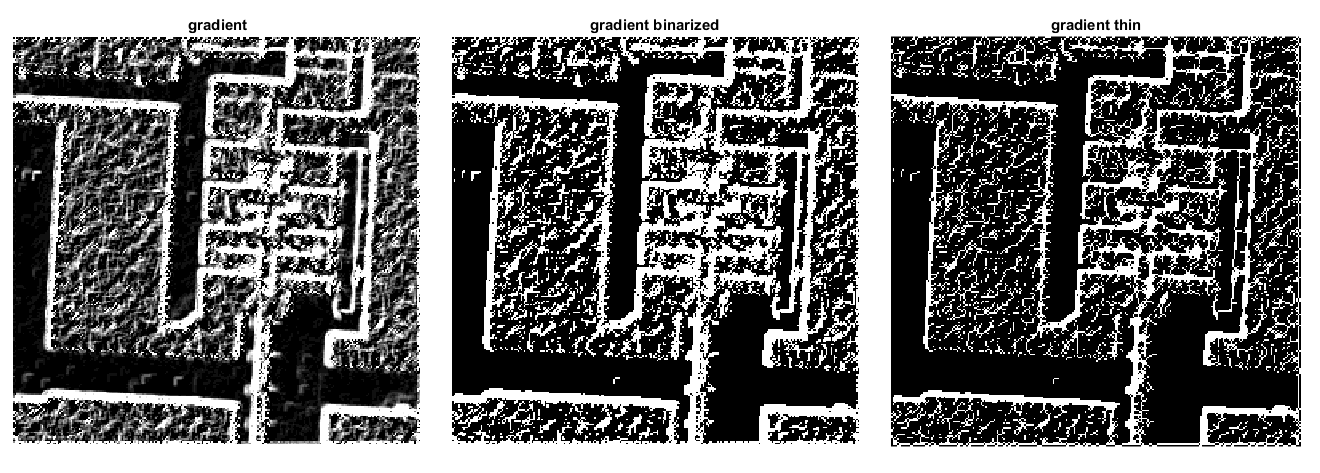
\includegraphics[width=\linewidth]{images/gradient.png}
		\end{figure}
		
		\paragraph{Laplacian filter\\}
		The second filter we used is the Laplacian. Zero crossings of the Laplacian are more accurate than gradient at localizing edges as can be seen after applying again \textit{im2bw()} and \textit{bwmorph()}.
		\begin{lstlisting}
			laplacian=imfilter(img_f,fspecial('laplacian'));
			laplacian=im2bw(laplacian,graythresh(laplacian)); 
			laplacian=bwmorph(laplacian,'thin');
		\end{lstlisting}
		\begin{figure}[h!]
			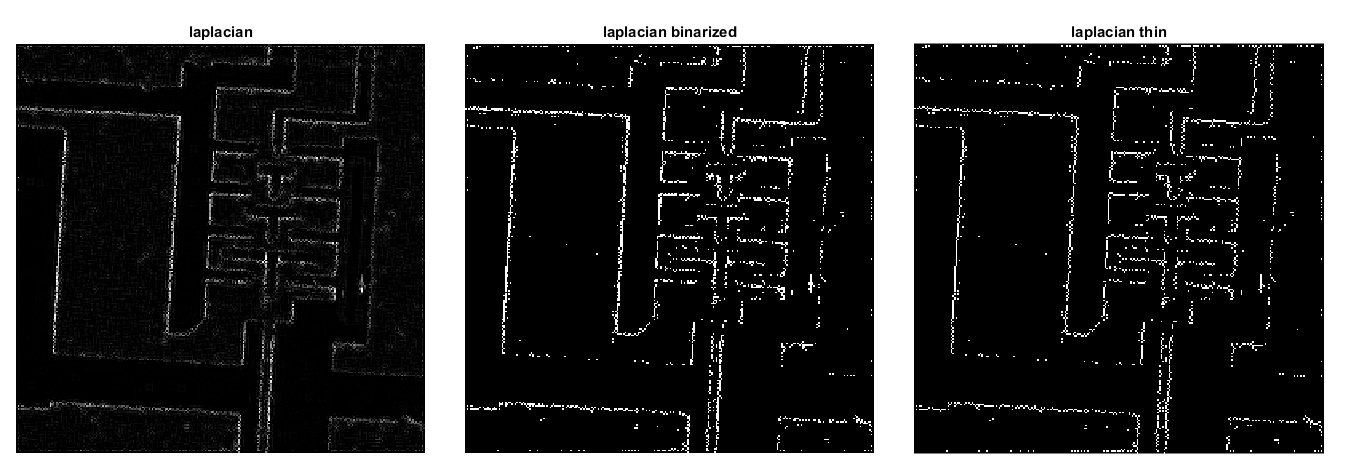
\includegraphics[width=\linewidth]{images/laplacian.png}
		\end{figure}
		\paragraph{Canny edge detector\\}
		The last technique we used is the Canny edge detector. After some tests we found an optimal threshold value of 0.4. This method does not require neither binarization nor morphological operations.
		\begin{lstlisting}
			canny=edge(img_f,'canny', 0.4);
		\end{lstlisting}
		Comparing the different results it can be immediately seen how the Canny's method gives a clearer result.
		\begin{figure}[H]
			\centering
			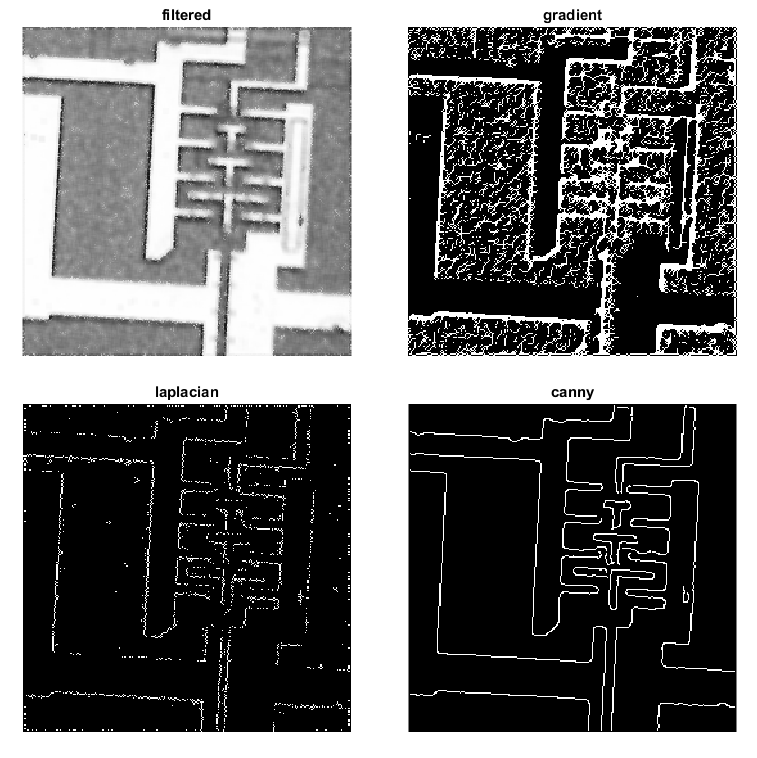
\includegraphics[width=.81\linewidth]{images/edge_detect.png}
		\end{figure}
		
		\subsubsection*{Step 4: compute the Radon transform}
		\par
		To compute the Radon transform we used the function \textit{radon()}. The relation between the transform and the edge image has been analysed by means of the function \textit{interactiveLine()} on step 5.
		\vspace{\baselineskip}
		\newline
		\textit{How does the Radon transform relate to the Hough trasform for lines?}
		\vspace{0.5\baselineskip}
		\begin{adjustwidth}{0.5cm}{}
			The Radon transform and the Hough transform are strictly related when doing line detection, we could say that the former is a simplified version of the latter.
			\newline
			The main difference between the two transformations is in the mathematical formulation, while the Hough transform is a discrete algorithm, the Radon transform is defined as an integral.
			\newline
			The Radon transform is also easier to understand from a conceptual point of view: it projects the whole image over an axis rotating from 0 to 179 degrees. The Hough transform instead takes one or more features (pixels) from the image and associates it to one or more parametric curves in the Hough space.
		\end{adjustwidth}
		\vspace{\baselineskip}
		\textit{Why the sum over any column of the Radon transform is always the same?}
		\vspace{0.5\baselineskip}
		\begin{adjustwidth}{0.5cm}{}
			The sum corresponds to the amount of information of the image, it is constant because each column contains the entire projection. For example, if we make the Radon transform of an horizontal line we'll notice that the vector corresponding to 0 degrees has uniform distributed values while the column corresponding to 90 degrees has a unique peak whose value is equal to the sum of all the values of the horizontal projection.
		
		\end{adjustwidth}
	\section*{{\small Part \#3} \\ Post-processing: high level detection and\linebreak interpretation}
		\subsubsection*{Step 5: choose points in Radon transform and observe associated lines}
		\par
		Using the function \textit{interactiveLine()} we can understand the relation between the points in the Radon space and the lines in the image.
		It can be noticed that each point in the image corresponds to a sinusoid in the transform domain and the main lines of the image (the edges) correspond to the intersection points between beams of sinusoids, because these sinusoids are the transform of the points belonging to the same line.
		\begin{figure}[H]
			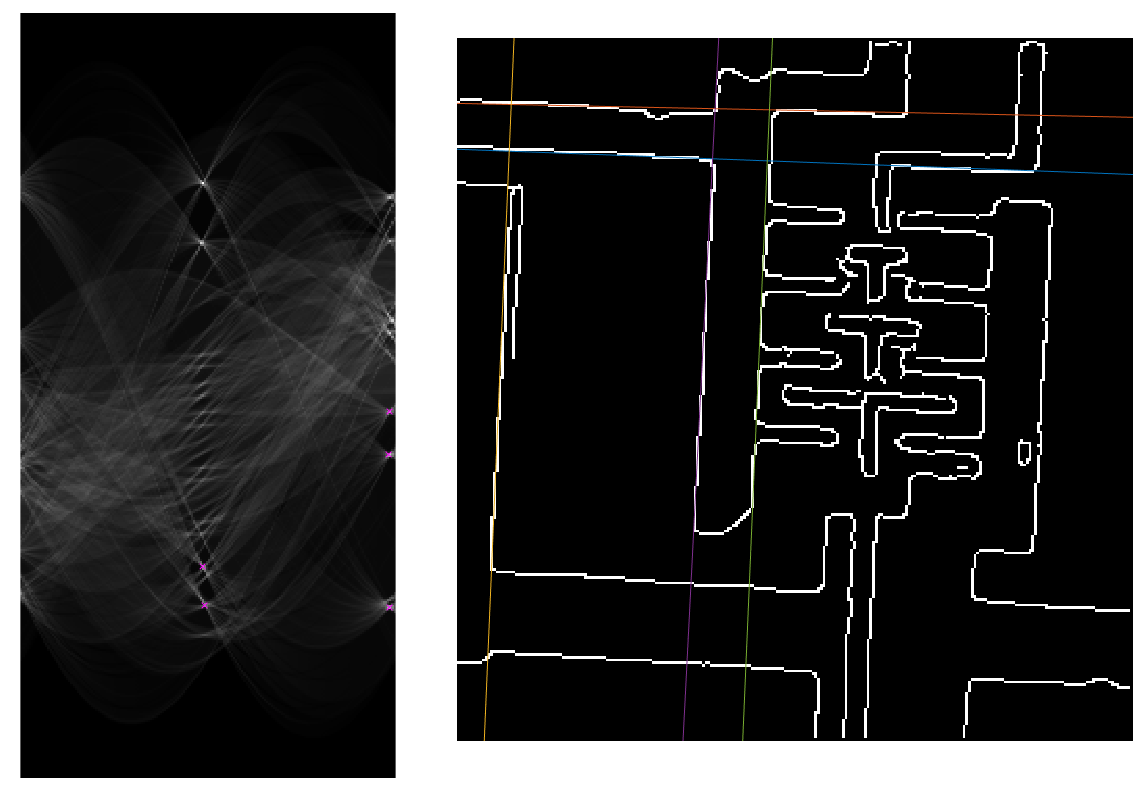
\includegraphics[width=\linewidth]{images/interactive_lines.png}
		\end{figure}
		
		\subsubsection*{Step 6: find the image orientation and rotate it}
		\par
		To find the image orientation we need to find the most significant columns in the Radon transform. In order to do this we compute the maximum value of each column of the matrix \textit{rad} and we save it in the vector \textit{high}.		
		\begin{lstlisting}
			rad=radon(edges);
			
			high=zeros(1,180);
			for i=1:180
				high(i)=max(rad(:,i));
			end
		\end{lstlisting}
		\vspace{0.5\baselineskip}
		Since we want to find two main (orthogonal) directions we need to look for the maximum value of the sum of the two parts of the \textit{high} vector, from 0 degrees to 89 and from 90 degrees to 179.
		\begin{lstlisting}
			maxsum=max(high(1:90)+high(91:180));
			indexsum=find(high(1:90)+high(91:180)==maxsum);
			
			img_rot=imrotate(img_f,90-indexsum,'bicubic');
		\end{lstlisting}
		\begin{figure}[H]
			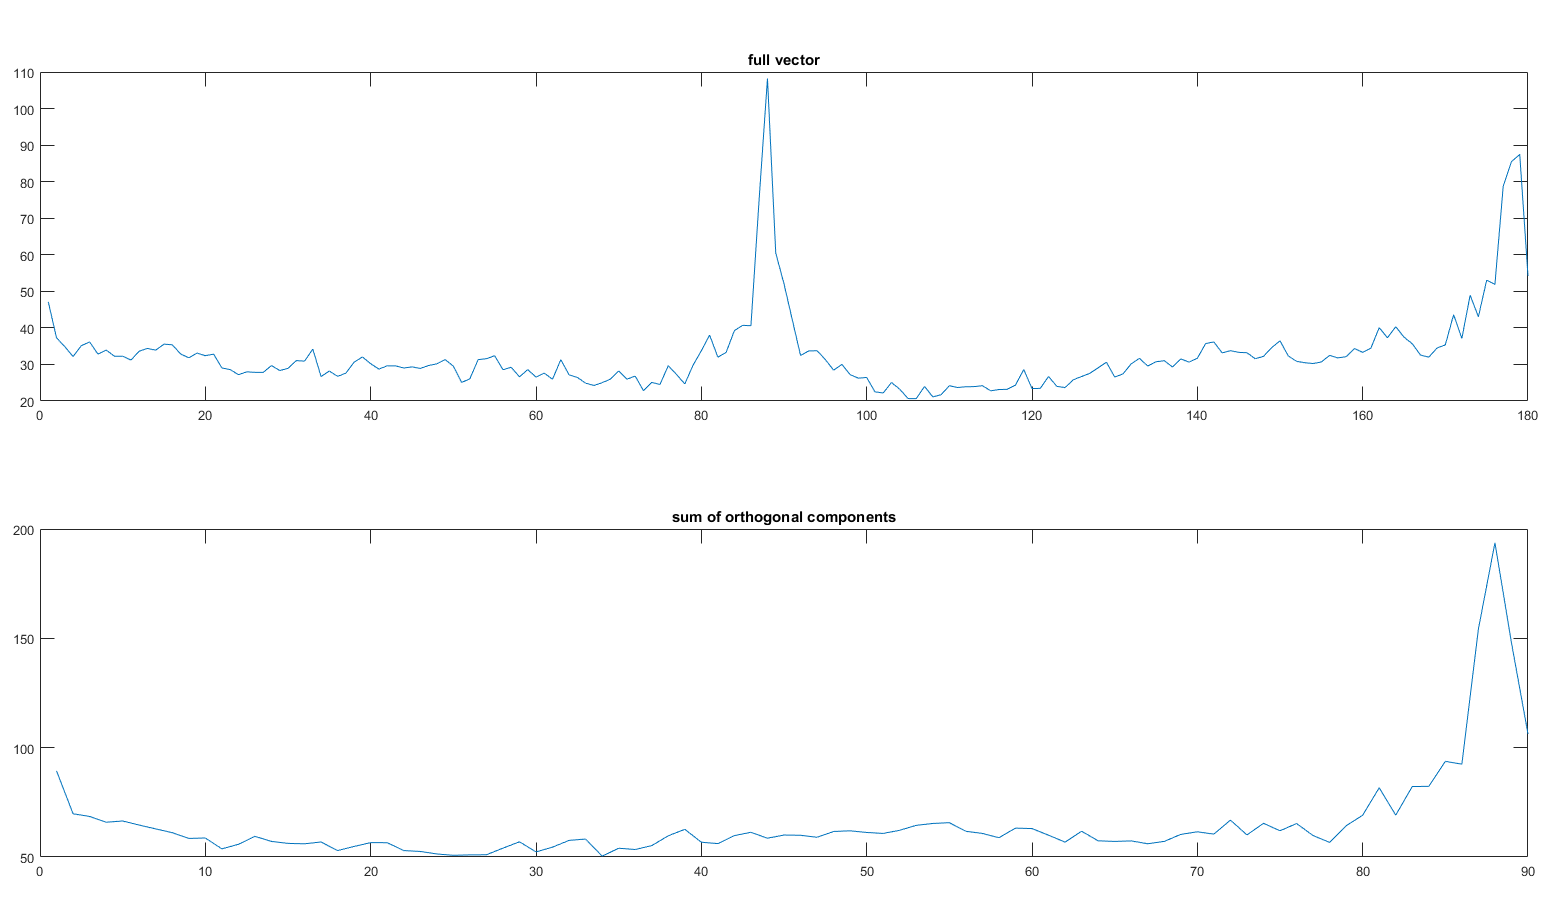
\includegraphics[width=\linewidth]{images/vector_plot.png}
		\end{figure}
		The orientation of the image corresponds to the index of the greatest value in the vector therefore to align the image we need to rotate it by \textit{90 - index} degrees.
		\begin{figure}[H]
			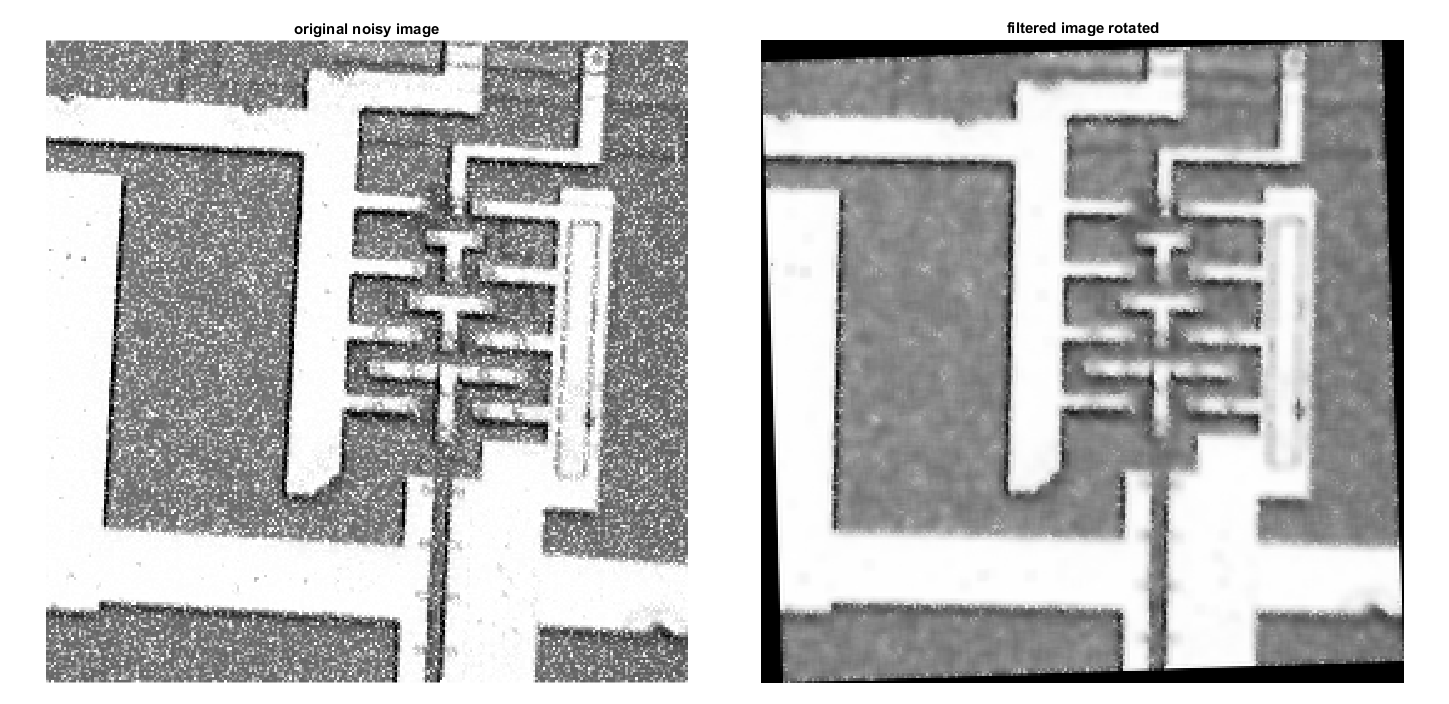
\includegraphics[width=\linewidth]{images/final_result.png}
		\end{figure}
	\section*{Final remarks}
	\par
		When we increase the noise we lose the sharpness of the image also after preprocessing but the computation of the rotation angle is not influenced because the Canny method is able to detect edges anyway.
		\newline
		By increasing the size of the filter we can decrease the amount of noise but the image may become too blurred and it is possible to lose some segments of the edges.
		\begin{figure}[H]
			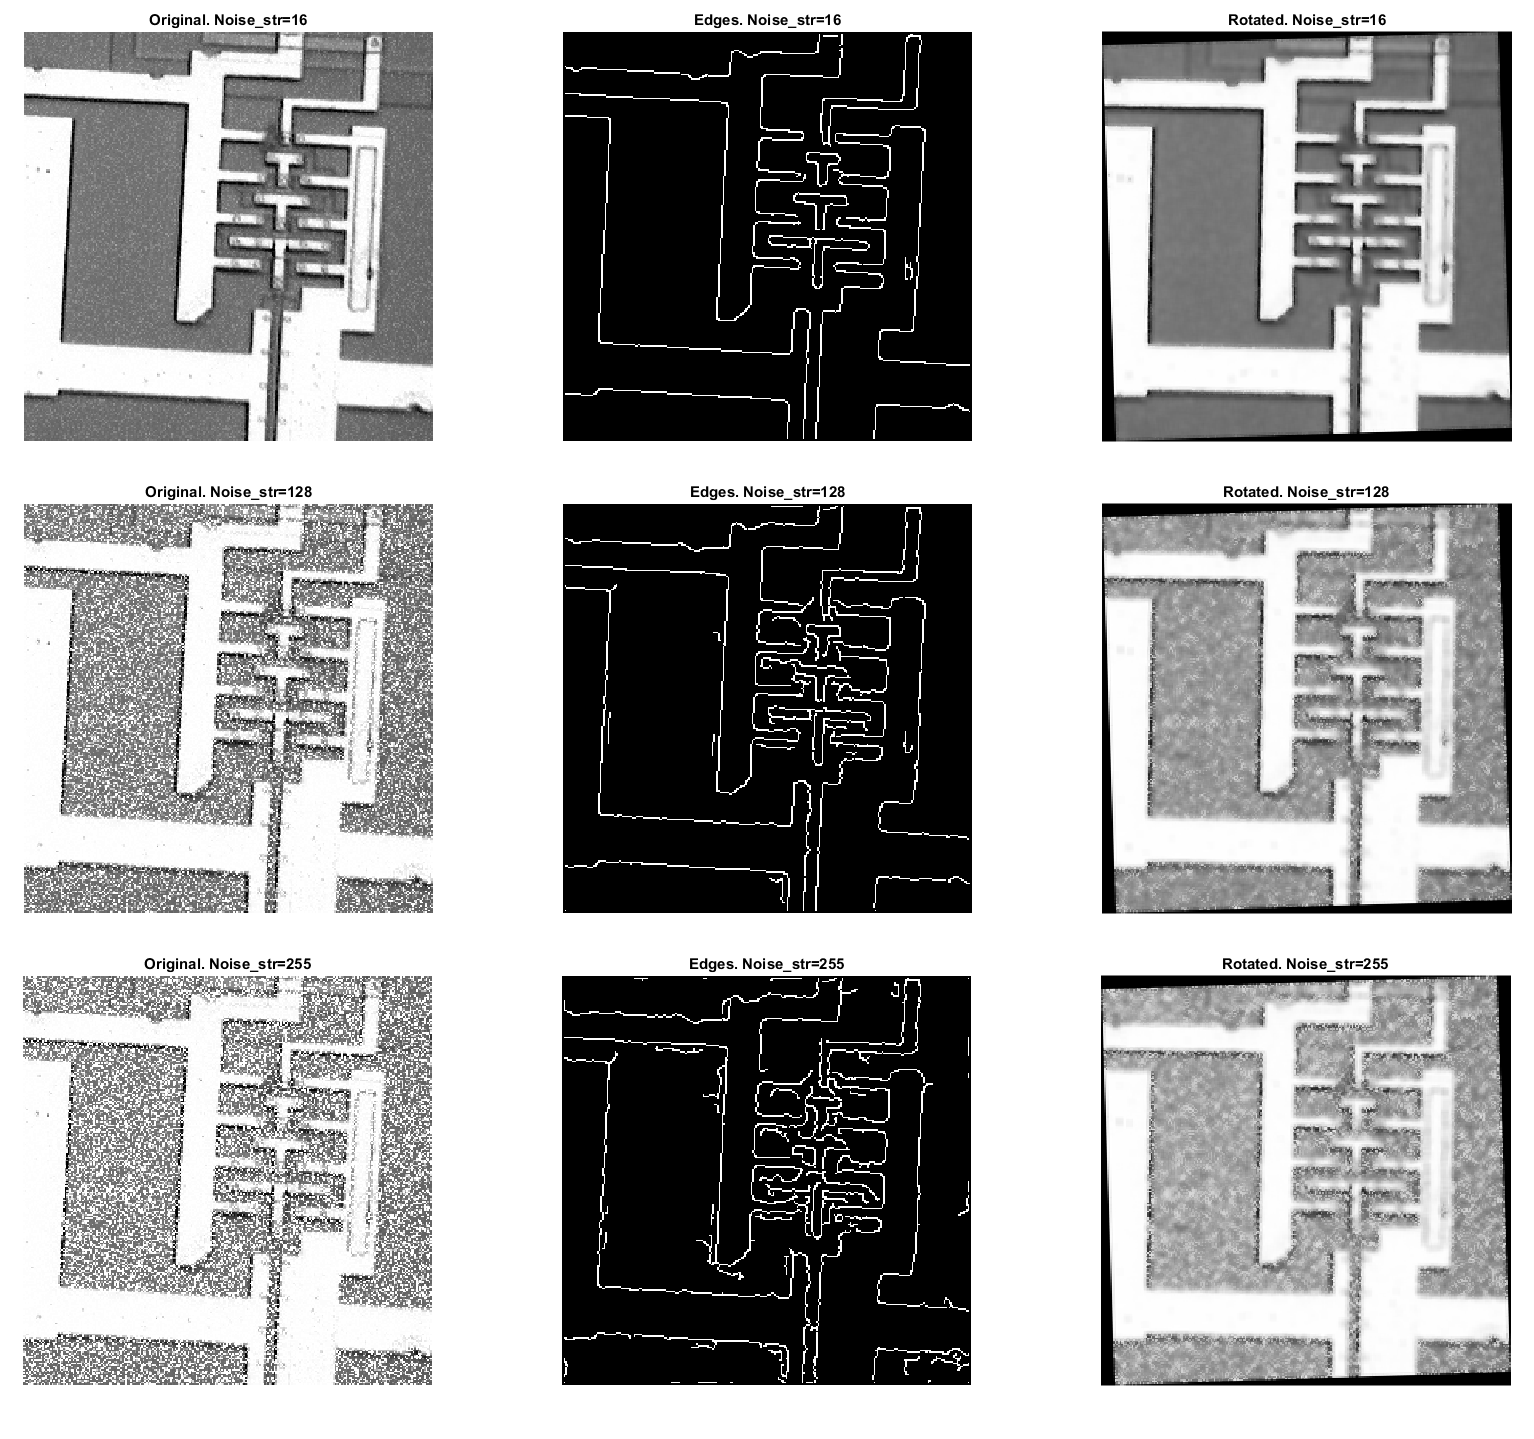
\includegraphics[width=\linewidth]{images/noise_comp.png}
		\end{figure}
\end{document}